\centerline{
\begin{minipage}{1.3\textwidth}
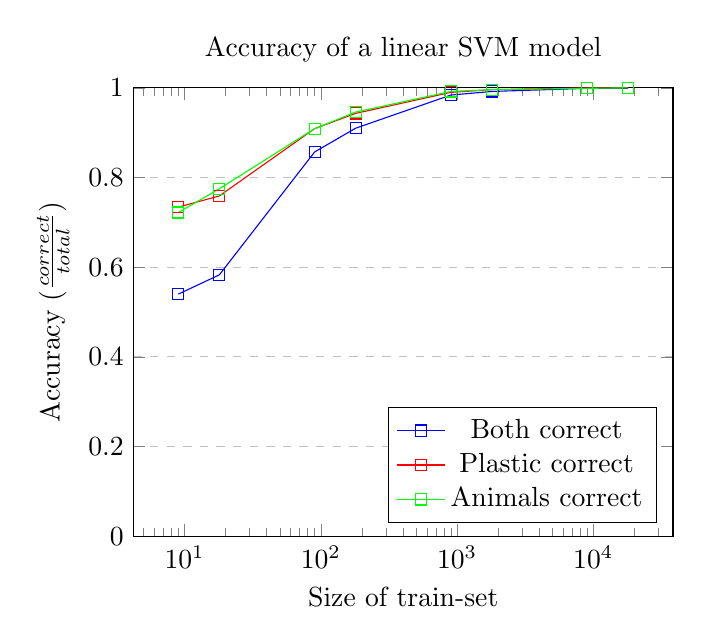
\begin{tikzpicture}
\begin{semilogxaxis}[
    title={Accuracy of a linear SVM model},
    xlabel={Size of train-set},
    ylabel={Accuracy ($\frac{correct}{total}$)},
    %xmin=0, xmax=18000,
    ymin=0, ymax=1,
    legend pos=south east,
    ymajorgrids=true,
    grid style=dashed,
]
\addplot[
    color=blue,
    mark=square,
    ]
    coordinates {
    %(14,0.571)(140,0.898)(1400,0.993)(14000,0.999)
     (9,0.540) (18,0.583) (90,0.857) (180,0.910) (900,0.984) (1800,0.992) (9000,0.999) (18000,0.999)
    };
    \addlegendentry{Both correct}
\addplot[
    color=red,
    mark=square,
    ]
    coordinates {
    (9,0.734) (18,0.759) (90,0.909) (180,0.943) (900,0.990) (1800,0.996) (9000,1.000) (18000,1.000)
    %(14,0.741)(140,0.947)(1400,0.996)(14000,1.000)
    };
    \addlegendentry{Plastic correct}
\addplot[
    color=green,
    mark=square,
    ]
    coordinates {
    (9,0.722) (18,0.775) (90,0.909) (180,0.946) (900,0.992) (1800,0.996) (9000,0.999) (18000,1.000)
    %(14,0.766)(140,0.924)(1400,0.997)(14000,0.999)
    };
    \addlegendentry{Animals correct}
\end{semilogxaxis}
\end{tikzpicture}
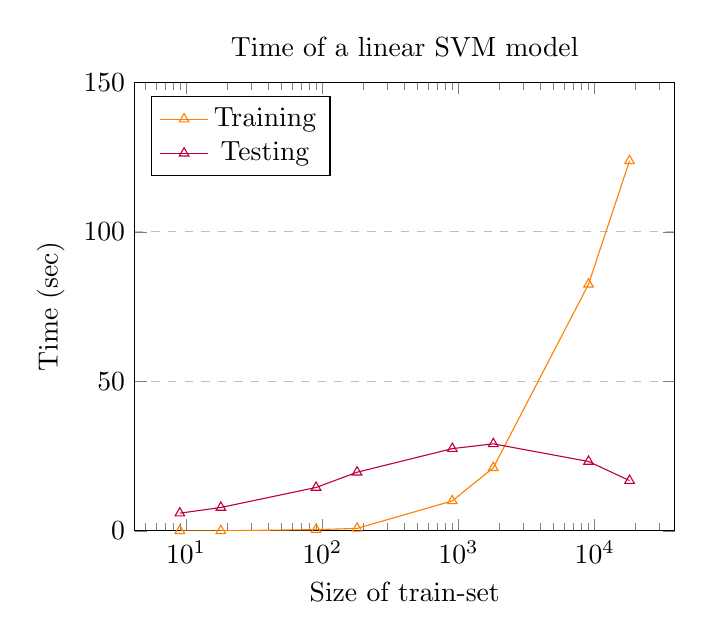
\begin{tikzpicture}
\begin{semilogxaxis}[
    title={Time of a linear SVM model},
    xlabel={Size of train-set},
    ylabel={Time (sec)},
    %xmin=0, xmax=18000,
    ymin=0, ymax=150,
    legend pos=north west,
    ymajorgrids=true,
    grid style=dashed,
    ]
\addplot[
    color=orange,
    mark=triangle,
    ]
    coordinates {
    (9,0.0) (18,0.0) (90,0.4) (180,0.8) (900,10.0) (1800,21.1) (9000,82.5) (18000,123.8)
    %(14,0.0)(140,0.2)(1400,5.6)(14000,74.6)
    };
    \addlegendentry{Training}
\addplot[
    color=purple,
    mark=triangle,
    ]
    coordinates {
    (9,5.9) (18,7.8) (90,14.5) (180,19.6) (900,27.5) (1800,29.1) (9000,23.2) (18000,16.8)
    %(14,0.6)(140,3.1)(1400,8.3)(14000,8.4)
    };
    \addlegendentry{Testing} 
\end{semilogxaxis}
\end{tikzpicture}
\end{minipage}
}